\chapter{เอกสารและงานวิจัยที่เกี่ยวข้อง}
\label{chapter:related-theory}

\section{ทฤษฎีและเนื้อหาที่เกี่ยวข้อง}
\subsection{การบริหารจัดการทรัพยากรมนุษย์}
การบริหารจัดการทรัพยากรมนุษย์ (Human Resources Management) คือกระบวนการที่จัดการนำเป้าหมายของบุคลากรและเป้าหมายขององค์กรให้มาบรรจบกัน เพื่อผลสำเร็จร่วมกันของทั้งองค์กรและบุคคล โดยมุ่งเน้นไปที่ผลของการจัดการ ส่งเสริมและช่วยพัฒนาศักยภาพของพนักงงานอย่างเต็มความสามารถ
\subsection{กฎหมายคุ้มครองแรงงาน}
ตามกฎหมายคุ้มครองแรงงาน วันหยุดพักผ่อนประจำปี ต้องมีไม่ต่ำกว่า 6 วันต่อปีสำหรับลูกจ้างที่ทำงานติดต่อกันมาครบ 1 ปี และลูกจ้างสามารถ ลาป่วย ลากิจ ลาทำหมัน ลารับราชการทหาร ลาคลอดบุตร และลาฝึกอบรมได้

\section{เทคโนโลยีและภาษาที่ใช้ในการพัฒนา}
\subsection{HTML}
HTML ย่อมาจาก Hypertext Markup Language  คือภาษาสากลในการสร้างหน้า Web page
\begin{figure}[!h]
	\centering
	
\includegraphics[width=0.35\linewidth]{html}
	\caption{Hypertext Markup Language}
	\label{Fig:HTML}
\end{figure}
\newpage
\subsection{CSS}
CSS ย่อมาจาก Cascading Style Sheets เป็นภาษาจัดการหน้าตาให้กับเอกสาร ให้กับ Markup Language เช่่น HTML
\begin{figure}[!h]
	\centering
	
\includegraphics[width=0.25\linewidth]{css}
	\caption{CSS}
	\label{Fig:CSS}
\end{figure}

\subsection{TypeScript}
TypeScript เป็นภาษาสคริปที่มีพัฒนาต่อมาจากภาษา JavaScript ที่เพิ่ม Type System ที่สามารถกำหนดชนิดของตัวแปรได้
เพิ่มความสามารถในการเขียนโปรแกรมเชิงวัตถุ (Object Oriented Programming:OOP) ซึ่งจะทำให้การพัฒนาดเป็นได้ง่ายขึ้น
โดยภาษา TypeScript เป็น transpiler ที่แปลงโค้ดกลับไปเป็น JavaScript ทำให้สามารถทำงานร่วมกับภาษา JavaScriptได้
\begin{figure}[!h]
	\centering
	
\includegraphics[width=0.5\linewidth]{ts}
	\caption{TypeScript}
	\label{Fig:TypeScript}
\end{figure}

\subsection{React TypeScript}
React ถูกสร้างขึ้นโดย Facebook เป็น JavaScript library สำหรับสร้าง User interface และมี libraries ที่ช่วยจัดการด้านต่างๆมากมาย ซึ่งทำให้การพัฒนาเว็บไซต์เป็นไปง่ายขึ้น
และเขียนในรูปแบบ SPA (Single Page Application) และเป็น Client Side Rendering
โดยปกติ React จะติดตั้งค่าเริ่มต้นด้วยภาษา JavaScript จึงต้องเปลี่ยนตั้งค่าเป็น TypeScript เพื่อทำให้การพัฒนาง่ายขึ้น
\begin{figure}[!h]
	\centering
	
\includegraphics[width=0.5\linewidth]{react}
	\caption{React TypeScript}
	\label{Fig:react}
\end{figure}

\subsection{GraphQL}
GraphQL ถูกสร้างขึ้นโดย Facebook เป็น Query language หรือ ภาษาที่ใช้ในการสืบค้นข้อมูลจาก API เหมือนเป็นตัวกลางที่ใช้ในการจัดการข้อมูลต่างๆ โดยจะ Response กลับมาเป็น JSON สามารถเลือกรับเฉพาะข้อมูลที่ต้องการได้ เพื่อลดปริมาณ Data ในการรับส่งข้อมูล และสามารถเรียกข้อมูลจากหลาย resource จาก request เดียวได้
\begin{figure}[!h]
	\centering
	
\includegraphics[width=0.5\linewidth]{graphql}
	\caption{GraphQL}
	\label{Fig:graphql}
\end{figure}

\section{เครื่องมือที่ใช้ในการพัฒนา}
\subsection{Visual Studio Code}
Visual Studio Code: VS Code เป็นโปรแกรม source code editor ในหลายภาษา ที่มีความสามารถและเครื่องมือที่ช่วยเหลือในการพัฒนา เช่น ใช้ code refactoring, ตรวจสอบ syntax, debuging รวมทั้งมี Extension ที่สามารถติดตั้งเพิ่มเติมเพื่อช่วยให้การพัฒนามีความสะดวก รวดเร็วและลดความผิดพลาด
\begin{figure}[!h]
	\centering
	
\includegraphics[width=0.20\linewidth]{vscode}
	\caption{Visual Studio Code}
	\label{Fig:vscode}
\end{figure}
\subsection{Git}
Git เป็น version control ที่เป็นระบบที่ใช้จัดเก็บติดตาม และควบคุมการเปลี่ยนแปลงที่เกิดขึ้นกับไฟล์ชนิดใดก็ตาม ช่วยให้การพัฒนางานในทีมเป็นไปอย่างมีระบบ คนในทีมสามารถใช้โค้ดที่เป็นเวอร์ชั่นล่าสุดตลอดเวลา หรือสามารถแก้ไขและแยกสายการพัฒนา (Branch) ออกมาได้
\begin{figure}[!h]
	\centering
	
\includegraphics[width=0.4\linewidth]{git}
	\caption{Git}
	\label{Fig:git}
\end{figure}
\subsection{Cloud Build}
Cloud Build คือบริการของ Google ที่ช่วย Build, test และ Deploy อัตโนมัติโดยสามารถตั้งทริกเกอร์ให้ทำงานทุกครังที่ push ขึ้นไปได้
\subsection{Firebase}
Firebase ถูกสร้างขึ้นโดย Google เป็น Platform ที่มีบริการเครื่องมือช่วยเหลือ การพัฒนาแอปพลิเคชัน ในรูปแบบ Serverless โดยมีทั้งแบบใช้ฟรีและ เสียเงินตามที่ใช้ โดยในโปรเจคนี้ได้ใช้บริการเครื่องมือของ Firebase ได้แก่ Cloud Firestore
\begin{figure}[!h]
	\centering
	
\includegraphics[width=0.5\linewidth]{firebase}
	\caption{Firebase}
	\label{Fig:firebase}
\end{figure}
\subsubsection{Cloud Firestore}
Cloud Firestore เป็นบริการจัดเก็บข้อมูลโดยโครงสร้างจะเป็นแบบ NoSQL ที่สามารถจัดเก็บข้อมูลในรูปแบบ Document ที่จะผูก Fields กับ Values เข้าด้วยกัน
ซึ่ง Document ก็จะถูกจัดเก็บใน Collections อีกที และสามารถสร้าง SubCollections ใน Document ได้ต่อไปเรื่อยๆ และยังสามารถช่วยเรื่องจัดเรียงข้อมูล (Sorting), การกรองข้อมูล (Filtering), การจำกัดข้อมูล (Limits) และการแบ่งหน้าข้อมูล (Paginate) เป็นต้น
\subsubsection{Firebase Hosting}
Firebase Hosting เป็นบริการ Web Hosting ใช้ในการ deploy เว็บไซต์ขึ้นไปบน Server ให้สามารถเข้าใช้ได้ผ่านทาง Internet รองรับทั้งเว็บไซต์ Static และ Dynamic และมี SSL (Secure Socket Layer) ให้ฟรี

\subsection{Google analytics}
Google analytics ถูกสร้างโดย Google เป็นเครื่องมือสำหรับเก็บสถิตการเข้าเว็บไซต์ และระบุว่าผู้ใช้เข้าเว็บไซต์จากประเทศใด ช่วงเวลาใด และเข้าถึงหน้าใดบ้าง
\begin{figure}[!h]
	\centering
	
\includegraphics[width=0.7\linewidth]{google-analytics}
	\caption{Gatsby}
	\label{Fig:gatsby}
\end{figure}

\subsection{Gatsby}
Gatsby เป็น Open source Framework โดยมีพื้นฐานมาจาก React โดยสามารถทำ SSR (Server Side Rendering)
ได้ทำให้การรองรับ SEO และถูก Google search มองเห็นมากขึ้น

\begin{figure}[!h]
	\centering
	
\includegraphics[width=0.7\linewidth]{gatsby}
	\caption{Gatsby}
	\label{Fig:gatsby}
\end{figure}

\subsection{Ant design}
Ant Design เป็น Open source UI Framework ในการสร้าง Components สำเร็จรูป ทำให้ไม่เสียเวลาในการสร้างใหม่
ก่อตั้งและพัฒนาภายในประเทศจีน รองรับทั้ง React, Angular และ Vue ที่เป็น Web Framework สำหรับการพัฒนาเว็บไซต์
\begin{figure}[!h]
	\centering
	
\includegraphics[width=0.7\linewidth]{ant-design}
	\caption{Ant Design}
	\label{Fig:ant-design}
\end{figure}
\subsection{Apollo}
Apollo เป็น Open source Platform สำหรับพัฒนา APIs ในชั้น communication layer 
โดยใช้ GraphQL Language ในการติดกันระหว่าง 2 ด้าน และมีเครื่องมือช่วยเหลือทั้งด้าน Client (Frontend) และ Server (Backend)

\begin{figure}[!h]
	\centering
	
\includegraphics[width=0.5\linewidth]{apollo}
	\caption{Apollo}
	\label{Fig:apollo}
\end{figure}
\subsubsection{Appollo Client (React)}

\subsubsection{Apollo Server}

\subsection{Formik}
เขียนดีไหมวะ


\section{ลักษณะขั้นตอนการทำงาน}
\subsection{Sprint planning}
ทีมจะมีประชุมวางแผนในการจัดสรรงาน (Task) ตาม Sprint backlog ที่ส่วนนี้ทาง System Analyst ได้กำหนดขึ้นมาก่อนแล้ว เมื่อแบ่งงานเสร็จจะมีการประเมินเวลาในการทำงานให้เหมาะสม โดยงานและการประเมินเวลาของแต่ละงาน จะมีการบันทึกลงใน Sprint task board ของ Taiga ซึ่งเป็น Project management tools ที่ทำให้ทุกคนในที่มสามารถติดตามกิจกรรมต่างๆได้ตามรูปที่ \ref{Fig:taiga}
\subsection{Gitflow}
เป็นการใช้ \textbf{Git} ที่เป็นเครื่องมือจัดการ Code collaboration และ Version control โดยแยก Branch เป็น Master Develop และ Feature โดยทีมเลือกใช้บริการ Git ของ \textbf{Bitbucket}

\textbf{Master Branch}\\
เป็น Branch ของ code Production จะเป็นตัวที่ทำการ test และแก้ไขมาเรียบร้อยแล้ว

\textbf{Develop Branch} \\
เป็น Branch ที่ยังอยู่ในการพัฒนา ยังอยู่ในขั้นตอน Test และแก้ไขอยู่ หรือรอเวลาที่จะ Merge รวมเข้ากับ Master Branch หลัง Review เพื่อขึ้น Production

\textbf{Feature Branch}\\
เมื่อจำนวนผู้พัฒนามากขึ้น การพัฒนาใน Develop Branch อาจทำให้ Code ของ มีปัญหากันได้ จึงแยก Branch ไปตาม Feature เช่น feature/daily\_task feature/new\_calendar เมื่อทำเสร็จสิ้น merge รวมเข้ากับ Develop Branch



\subsection{Daily Scrum}
เป็นการบอกความเคลื่อนไหวของงานที่ตนเองได้รับ เพื่อแจ้งความคืบหน้า และแจ้งปัญหาที่ตนเองพบรวมถึงการแจ้งสิ่งทีตนเองได้ทำเสร็จสิ้นไปของเมื่อวาน ให้คนในทีมรับทราบ และช่วยกันแก้ไขปัญหา โดยปกติตามรูปแบบ SCRUM แล้วจะมีการทำ Standup meeting ที่คนในทีมต้องลุกขึ้นยืนและพูดคุยกัน แต่ Daily scrum ของที่บริษัทนี้จะใช้การส่งข้อความลงในแอพลิเคชั่น Slack ดังรูปที่ \ref{Fig:slack}

\subsection{Code review}
เป็นการประเมินการเขียนโปรแกรมเพื่อวิเคราะห์ข้อดี ข้อเสียของโครงสร้างและการทำงานของโปรแกรมที่ได้เขียนไปตลอด Sprint ที่ผ่านมา เพิ่อนำไปปรับปรุงและแก้ไขใน Sprint ถัดไป ในการปฎิบัติจริงกิจกรรมนี้จะทำในช่วง 2-3 สัปดาห์แรกของการปฎิบัติงาน เพิ่อให้มีลักษณะการเขียนโปรแกรมที่สอดคล้องกับคนในทีม หลังจากนั้นจึงมีการประเมินในบางครั้ง

\subsection{Sprint review}
ในช่วงวันสุดท้ายของแต่ละ Sprint จะมีการประชุมเพื่อสรุปสิ่งที่แต่ละคนในทีมได้ทำไป ย้ายงานที่ใช้ระยะเวลานานมากกว่า 1 Sprint ไปไว้ใน Sprint หน้า และพูดถึงปัญหาที่เกิดตลอด Sprint ที่ผ่านมาเพื่อนำไปปรับปรุงในการทำงาน Sprint ถัดไป

\
\begin{figure}[!h]
	\centering
	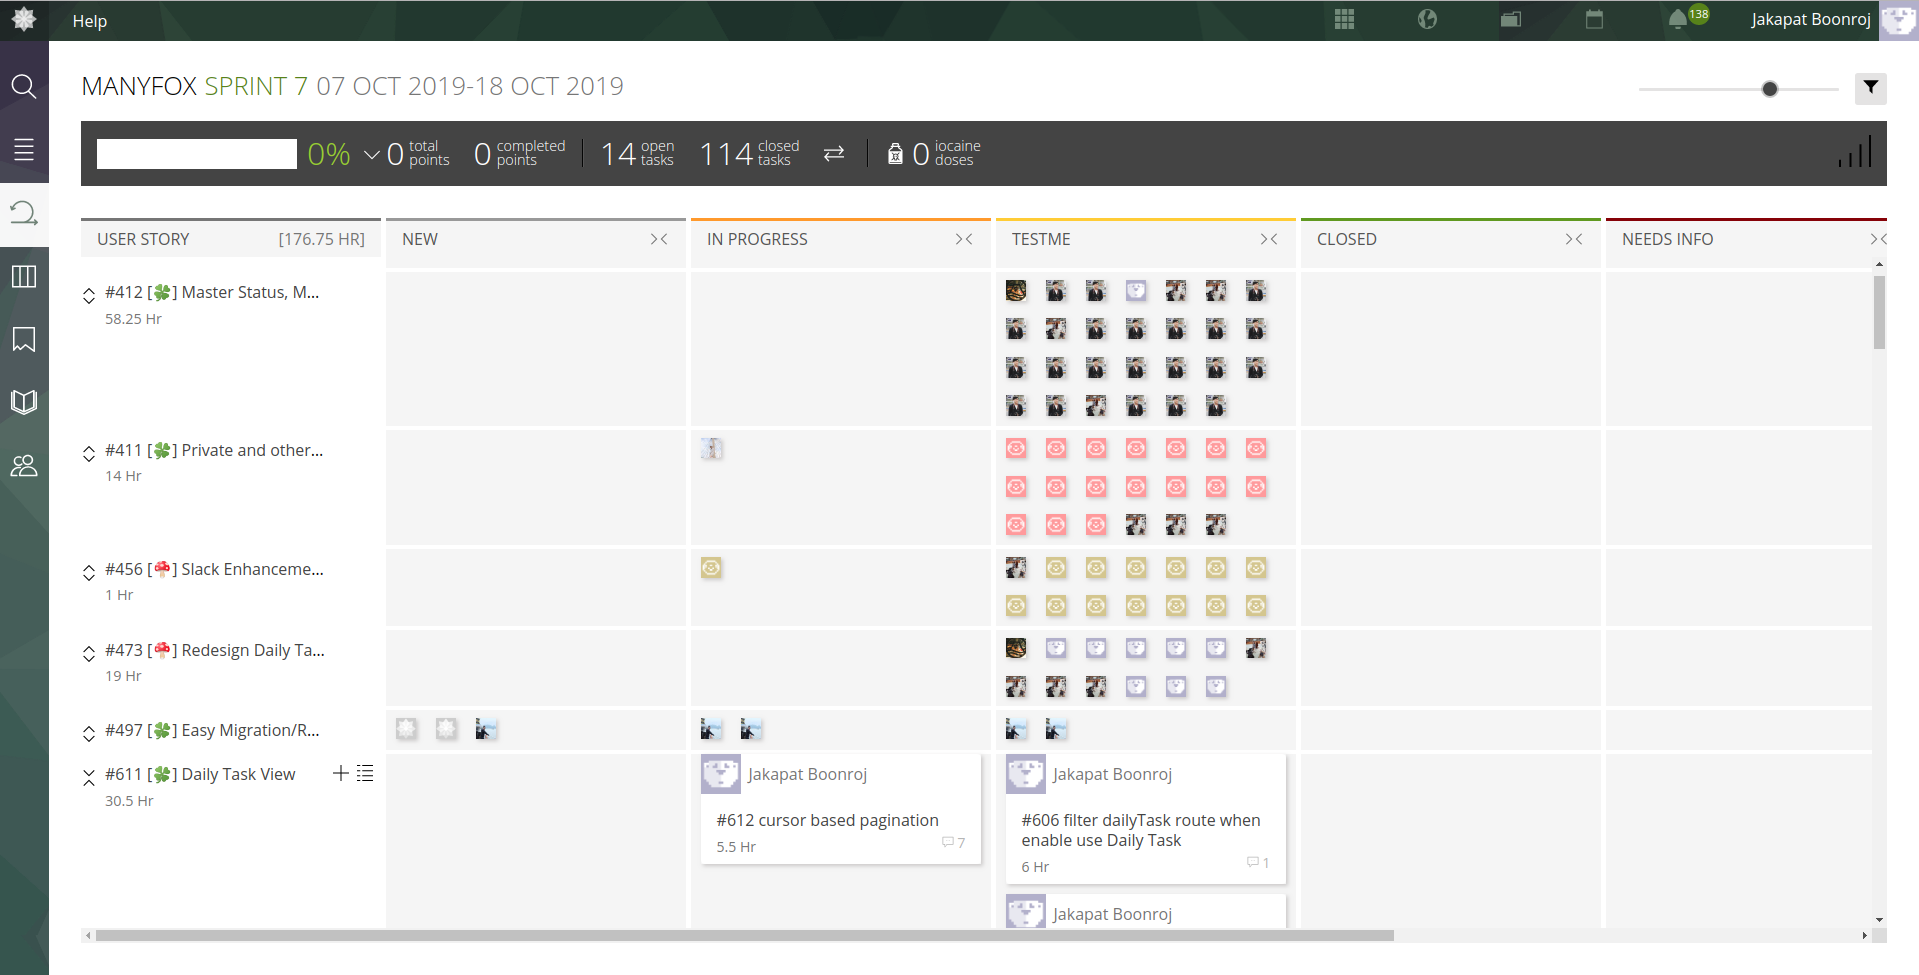
\includegraphics[width=0.8\linewidth]{taiga}
	\caption{Sprint task board ใน Taiga}
	\label{Fig:taiga}
	\centering
	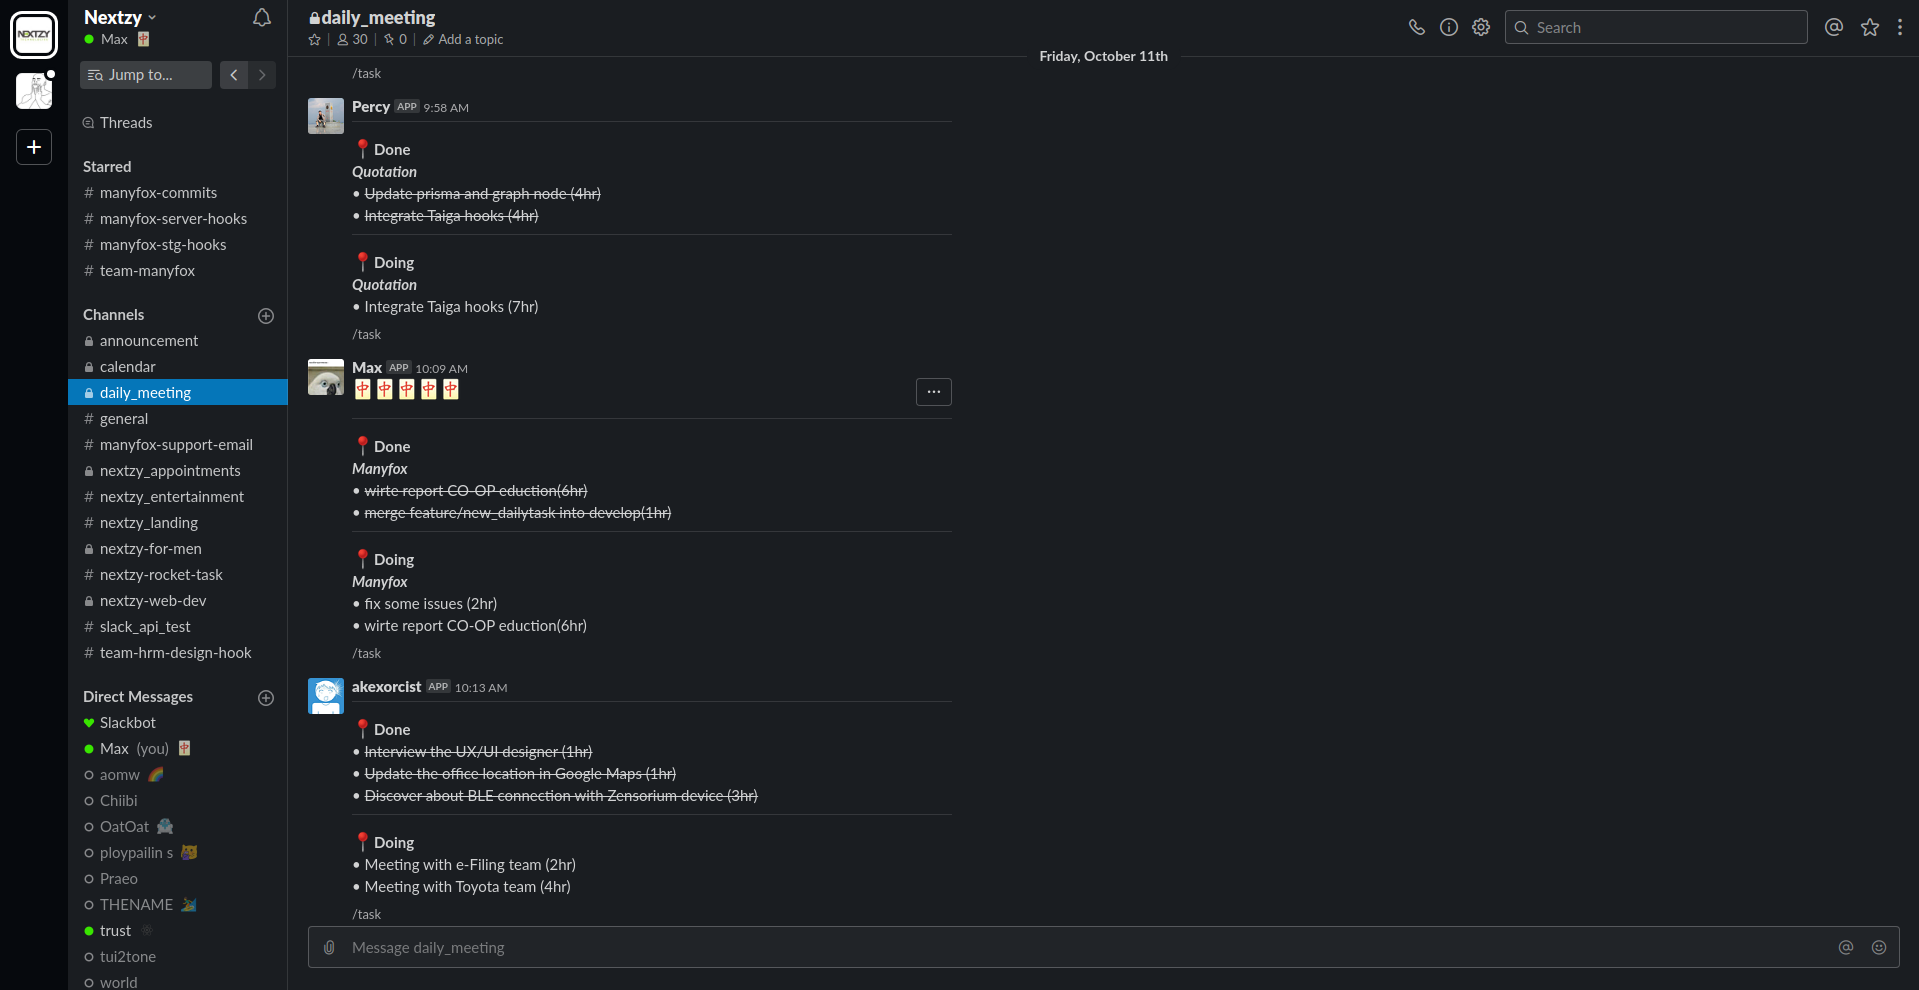
\includegraphics[width=0.8\linewidth]{slack}
	\caption{Daily meeting ใน Slack}
	\label{Fig:slack}
\end{figure}